\chapter{Introduction}

\begin{figure}
\begin{center}
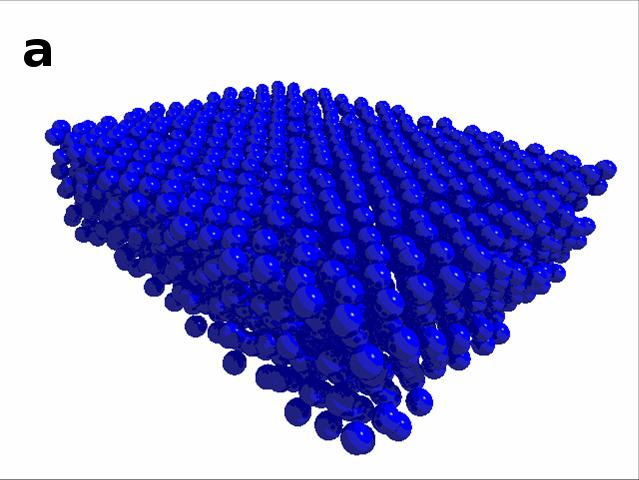
\includegraphics[height=1.5in]{figures/literature-review/sphere-crystal.png}
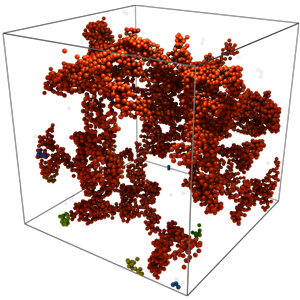
\includegraphics[height=1.5in]{figures/literature-review/sphere-gel.png}
\end{center}
\caption{Spherical colloids with purely repulsive interactions assemble into (a) ordered 
crystal structures with fcc geometry, while spheres with
attractive interactions may assemble into (b) open ``gel'' structures.}

\label{fig:isotropic-structs}

\end{figure}

As a class of materials, colloidal suspensions are of interest both
in the study of self-assembly~\cite{glotzer-solomon} in applications such
as photonic crystals~\cite{vos-photonic, yang-photonic} and three-dimensional templates for tissue 
engineering scaffolds~\cite{zhang-tissue}. However, despite the wide interest in these materials, the range of possible 
structures made available by the 
self-assembly of isotropically-interacting spherical colloids is relatively narrow.  Due to the isotropic nature
of colloidal interactions, there are only two assembled structures available.
When the interparticle interaction is purely 
repulsive, such as in a hard-core interaction,  a stable, ordered face-centered-cubic crystal
structure(Fig.~\ref{fig:isotropic-structs}(a)) with a volume fraction of 0.74 is formed.~\cite{ise-crystal, wong-crystal}
When the interparticle interaction is attractive, the particles may form an open, disordered ``gel'' 
structure (Fig~\ref{fig:isotropic-structs}(b)) 
with an essentially random arrangement and gap volumes which are potentially larger than the 
particle size.~\cite{warren-gel}

Many applications, such photonic crystals, would benefit from the availability of different
kinds of self-assembled structures.~\cite{glotzer-solomon}  One way to address this need is to 
introduce colloidal particles that incorporate one or more forms of anisotropy, in which the 
particle is altered such that the interaction between two or more particles becomes non-uniform depending on 
their relative orientations.  These alterations may be based on the shape of the particles, the chemical makeup
of the particles, or 
some combination of the two.

\begin{figure}[h]
\begin{center}
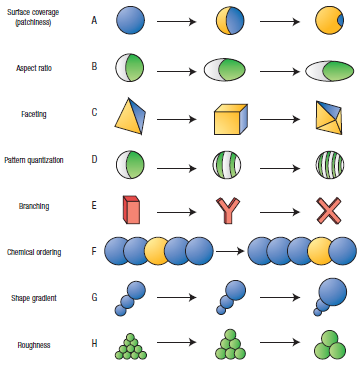
\includegraphics{figures/glotzer-anisotropy-dimensions.png}
\end{center}
\caption{Anisotropy dimensions proposed by Glotzer and Solomon~\cite{glotzer-solomon} to classify 
different forms of particle anisotropy.}
\label{fig:glotzer-dimensions}
\end{figure}


% Find many of the references in the following paragraph in Glotzer and Solomon's 2007 NatMat paper.
In a 2007 article in \textit{Nature Materials}~\cite{glotzer-solomon}, Glotzer and Solomon propose the system of anisotropy 
classification shown in Fig.~\ref{fig:glotzer-dimensions}. These 
anisotropy dimensions include shape-based dimensions such as aspect 
ratio, faceting, branching, shape gradient, 
and roughness (Fig.~\ref{fig:glotzer-dimensions}(B,C,E,G,H)), as well as dimensions based on the presence of
multiple chemistries such as surface coverage, pattern quantization, and chemical ordering 
(Fig.~\ref{fig:glotzer-dimensions}(A,D,G)).  These dimensions do not necessarily 
represent an exhaustive classification of the types
of anisotropy which are theoretically possible, but 
instead generalize from anisotropy types which have been observed in the
recent literature.  For example, rod-shaped or ellipsoidal particles of moderate aspect ratio have been fabricated 
by a wide variety of techniques including 
lithography~\cite{desimone-shear} and the stretching of colloidal spheres~\cite{rods-mohraz}; branched 
tetrapods have been fabricated of gold~\cite{gold-tetrapods},
and CdTe~\cite{cdte-tetrapods}; and chemically patterned particles have been produced
through microfluidic means~\cite{shepherd-janus}
as well as by conventional photolithography.~\cite{desimone-janus}  This list of dimensions may therefore
be seen as a useful framework for classification: by combining multiple dimensions, more complex types of particles may be 
designed (Fig.~\ref{fig:dimensions-combined}), or a complex particle may be classified in terms of which dimensions it includes.
New forms of anisotropy may be identified as those which cannot be decomposed into dimensions already identified.

\begin{figure}[h]
\begin{center}
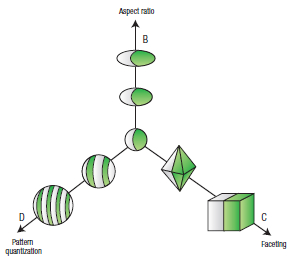
\includegraphics{figures/glotzer-combine-dimensions.png}
\end{center}
\caption{Multiple anisotropy dimensions may be combined to yield more complex forms.~\cite{glotzer-solomon}}
\label{fig:dimensions-combined}
\end{figure}

In this work, we develop techniques for
the fabrication of colloids with geometric and chemical anisotropy and begin to characterize the dynamical behavior
and self-assembly of these particles.

\section{Thesis Scope}

The aim of this work is to develop techniques for the fabrication and characterization of anisotropic colloids and to begin
to explore their dynamical and self-assembly behavior.  Fabrication is based on flow lithography
techniques for producing polymeric particles~\cite{dendukuri-cfl, dendukuri-sfl}, 
and characterization is primarily based on fluorescence and confocal 
microscopy~\cite{weitz-confocal} and particle 
tracking.~\cite{crocker-grier-spheres,rods-mohraz}
The systems used are based on a combination of a hydrophobic monomer (tri(methylol propane) triacrylate) and hydrophilic 
monomers (poly(ethylene glycol) diacrylate and 20-mol ethoxylated tri(methylol propane) triacrylate). 
Single-component particles are used to study the effects of
geometry on dynamical behavior in isolation, while multiple-component particles introduce 
the hydrophobic interaction to induce self-assembly.  Particles are suspended in a 
variety of solvents to explore this interaction, including
water, ethanol, dimethyl sulfoxide, isopropanol, and toluene.

\section{Thesis Organization}

Chapter~\ref{ch:comp-tracking}
details algorithms and software developed in the course of this study to analyze microscopy images containing 
anisotropic colloids.  Chapter~\ref{ch:rods} investigates the fabrication, behavior and self-assembly of simple rod-shaped colloids
in both single-component and ``Janus'' forms, while Chapter~\ref{ch:exotic} 
investigates colloids with more exotic geometries. The main
conclusions are presented in Chapter~\ref{ch:conclusions}.  
Appendix~\ref{sec:matlab-implementation} details the Matlab implementation of the algorithms developed in
Chapter~\ref{ch:comp-tracking}.
